\documentclass[a4paper,12pt]{article}
\usepackage[utf8]{inputenc}
\usepackage{amsmath}
\usepackage{amsfonts}
\usepackage{authblk}

% Customization
\usepackage{mathtools}
\DeclarePairedDelimiterX{\norm}[1]{\lVert}{\rVert}{#1}  % to use '\norm'
\newcommand{\quotes}[1]{``#1''}  % for quotes

% Graphics
\usepackage{graphicx}  % set up where images are stored
\graphicspath{ {./body/figures/} }
\usepackage{svg}

% Tables
\usepackage{tabularx}  % use tables with multi-line cells
\newcolumntype{C}{>{\centering\arraybackslash}X}
\newcolumntype{L}{>{\raggedright\arraybackslash}X}
\usepackage{makecell}

% For captions
\usepackage{caption}
\usepackage{subcaption}
%\captionsetup[table]{position=bottom} 

% Bibliography
\usepackage[style=nature, sorting=none, maxnames=5, minnames=5]{biblatex}
\addbibresource{sepsisLib.bib}
\DeclareNameAlias{sortname}{given-family}
%\bibliography{sepsisLib.bib}


\title{Continuous Sepsis Trajectory Prediction using Tensor-Reduced Physiological Signals}
% Author names
\author[1]{Olivia P. Alge*}
\author[1]{Joshua Pickard}
\author[1]{Winston Zhang}
\author[1]{Shuyang Cheng}
\author[2]{Harm Derksen}
\author[1,3,4]{Gilbert S. Omenn}
\author[5]{Jonathan Gryak}
\author[6,7,8,9]{J. Scott VanEpps}
\author[1,6,7,10]{Kayvan Najarian}

% Addresses & affiliations

% DCMB 
\affil[1]{Department of Computational Medicine and Bioinformatics, University of Michigan, Ann Arbor, MI, USA}

% Northeastern
\affil[2]{Department of Mathematics, Northeastern University, Boston, MA, USA}

% SPH
\affil[3]{School of Public Health, University of Michigan, Ann Arbor, MI, USA}

% Human Genetics
\affil[4]{Department of Internal Medicine and Human Genetics, University of Michigan, Ann Arbor, MI, USA}

%QC
\affil[5]{Department of Computer Science, Queens College, CUNY, Queens, NY, USA}

% MCIRCC
\affil[6]{Michigan Center for Integrative Research in Critical Care, University of Michigan, Ann Arbor, MI, USA}

% Emergency Medicine
\affil[7]{Department of Emergency Medicine, University of Michigan, Ann Arbor, MI, USA}

% BI
\affil[8]{Biointerfaces Institute, University of Michigan, Ann Arbor, MI, USA}

% Macromolecular Science and Engineering
\affil[9]{Macromolecular Science and Engineering, University of Michigan, Ann Arbor, MI, USA}

% Biomedical Engineering
%\affil[8]{Department of Biomedical Engineering, University of Michigan, Ann %Arbor, MI, USA}

% EECS
\affil[10]{Electrical Engineering and Computer Science, University of Michigan, Ann Arbor, MI, USA}

\affil[*]{Corresponding author email, phone number, and address: oialge@umich.edu; (734) 763-3924; NCRC 2800 Plymouth Rd. Bldg. 18-155, Ann Arbor, MI 48109}

% MIDAS
%\affil[9]{Michigan Institute for Data Science, University of Michigan, Ann Arbor, MI, USA}

\date{}

% some stuff for author affiliation script to work properly
\setcounter{Maxaffil}{0}
\renewcommand\Affilfont{\itshape\small}

% Start of document
\begin{document}

    \maketitle
    
    \clearpage
    
    \section*{Abstract} \label{sec:abstract}
    %should only be 250 words

The quick sequential organ failure assessment (qSOFA) scoring system is a method to determine which individuals are at risk to progress to poor outcomes related to sepsis using minimal variables. We used Support Vector Machine, Learning Using Concave and Convex Kernels, and Random Forest to predict an increase in qSOFA score using electronic health record (EHR) data, electrocardiogram, and arterial line.

A Random Forest model trained on ECG data alone shows an improved performance when tensor decomposition is used to reduce the feature space for predictions in a 6-hour time frame (AUROC 0.6690 $\pm$ 0.0644 compared to 0.5693 $\pm$ 0.0764). Adding waveform features from an arterial line can further improve performance (AUROC 0.6855 $\pm$ 0.0683), and the benefits of structuring the data as a tensor and performing tensor decomposition can still be seen (AUROC 0.7064 $\pm$ 0.0650). Lastly, adding EHR data features to a tensor-reduced signal model further improves performance (AUROC 0.7691 $\pm$ 0.0617).

Despite a reduction in performance going from an EHR data-informed model to a tensor-reduced waveform data model, the waveform-informed model offers distinct advantages. The first advantage of a signal features-based model is that predictions can be made on a continuous basis in real-time, and second is that these predictions would not be limited by the availability of EHR data. Additionally, structuring the waveform features as a tensor conserves structural and temporal information that would otherwise be lost if the data were presented as flat vectors.
    
    \section*{Introduction} \label{sec:intro}
    % State the objectives of the work and provide an adequate background, avoiding a detailed literature survey or a summary of the results.

% What are Sepsis and Septic shock?
Sepsis is a syndrome induced by an existing infection in the body that produces life-threatening organ dysfunction in a chain reaction. The clinical criteria for sepsis include suspected or documented infection and an increase in two or more Sequential Organ Failure Assessment (SOFA) points. Septic shock, a more severe subset, consists of substantially increased abnormalities \autocite{sepsis-3} and higher risk of mortality \autocite{paoli_epidemiology_2018}. It is imperative to risk-stratify patients early in their course in order to appropriately direct critical, but potentially limited, resources and therapies.

Sepsis' heterogeneity complicates its diagnosis and prognosis. Its current definition, based on SOFA score, requires measurement or collection of variables which may not be immediately available. The quick-SOFA (qSOFA) is a screening tool that can be performed at the bedside. It consists of three criteria - Glasgow Coma Scale of $<$ 15 (indicating mental status change), respiratory rate $\geq$ 22 breaths per minute, and systolic blood pressure $\leq$ 100 mmHg - where two of the three must be met \autocite{sepsis-3}. It includes the poorly characterized variable mental status change, but it is a better predictor of organ dysfunction than systemic inflammatory response syndrome (SIRS), which is less sensitive \autocite{sirs_1992, seymour_assessment_2016}. SIRS is the body's response to a stressor such as inflammation, trauma, surgery, or infection, while sepsis is specifically a response to infection; many septic patients have SIRS, but not all patients who meet SIRS criteria have an infection or experience septic organ failure. In comparison to qSOFA, SIRS has four criteria, three of which must be met to positively identify SIRS. These are: respiratory rate $>$ 20 breaths per minute or partial pressure of CO\textsubscript{2} $<$ 32 mmHg; heart rate $>$ 90 beats per minute; white blood cell count $>$ 12,000/microliter or $<$ 4,000/microliter or bands $>$ 10\%; and temperature $>$38$^{\circ}$C or $<$ 36$^{\circ}$C \autocite{sirs_chakraborty_systemic_2022}. For each of these scoring systems, factors such as comorbidities, medication, and age may confound the phenotype in different patient groups.

A system of sepsis detection which is too strict or time-consuming can delay necessary care to patients, and criteria that are too broad can lead to over-treatment or inappropriate use of limited resources. For example, false positive sepsis prognoses can lead to patients receiving unnecessary care and antibiotics, which contribute to antibiotic resistance and emergence of \quotes{superbugs} \autocite{vanepps_reducing_2018, prestinaci_antimicrobial_2015, chokshi_global_2019}. Similarly, qSOFA is not recommended as a single screening tool for diagnosis of sepsis \autocite{evans_surviving_2021}, but it can be used as a method of predicting prolonged ICU stay or in-hospital mortality \autocite{seymour_assessment_2016}. Predicting the trajectory of a patient with suspected infection may be a more efficient use of resources than detecting existing sepsis, and therefore trajectory prediction is the focus of this study. 

% on EHR data
Many models for detecting, monitoring, or predicting outcomes related to sepsis depend on Electronic Health Record (EHR) data, including SOFA score \autocite{sepsis-3}, EPIC's sepsis model \autocite{wong_external_2021}, and others \autocite{nesaragi_correlation_2021, morrill_signature_2019, taylor_prediction_2016}. EHR data can include static variables like demographics information, and dynamic variables such as vital signs or lab values. While useful for determining a patient's status, EHR data are limited by time. Lab values require time for collection and processing, and continuous variables may be updated less than hourly or at irregular intervals. In contrast, physiological readings, such as those generated from electrocardiography, blood pressure monitoring, or pulse oximetry, are collected continuously and at regular intervals. Our study examines the use of continuous physiological signals, namely electrocardiogram (ECG) and arterial line, in outcome prediction related to sepsis.

% on ECG data
ECG signal information has previously been used in the study of risk for sepsis and sepsis progression \autocite{berger_shock_2013, moorman_cardiovascular_2011, nemati_interpretable_2018}. The advantage that continuous monitoring devices like ECG offer over EHR data is real-time, continuous assessment of a patient's status. In addition, ECG is routinely collected in the intensive care unit (ICU), and is minimally invasive. In our analysis, we also include arterial line, as both SOFA and qSOFA use blood pressure to assess the status of a patient's cardiovascular system status \autocite{sepsis-3}.

% Why use tensors?
Given sepsis' complexity and heterogeneity, it is necessary to incorporate multiple variables into a trajectory prediction method. Modeling data as a tensor provides the ability to observe changes in different variables with respect to time and to one another. The prognosis and severity assessment of sepsis rely on a large amount of heterogeneous data, including body temperature, arterial blood pressure, blood culture tests, and molecular assays. Treatment of sepsis does not rely on any individual variable, but on all of these measurements, which vary as a function of time. Because no individual feature is sufficient, integrating data across time and incorporating structure is necessary for improved sepsis prognosis, and therefore can better inform care decisions.
% TODO: from Gil: "explain how tensor analysis achieves these benefits"

% transition to methods section
In this study, we use ECG and arterial line signals to predict an increase in an individual's qSOFA score, where a qSOFA of $\geq$ 2 indicates poor outcomes related to sepsis. The results of signal-trained models are then compared to models trained using both signals and EHR data. This is to (1) predict which individuals are at risk to decompensate to septic shock, experience future organ failure, or other complications related to sepsis, rather than focusing on a sepsis diagnosis, and (2) assess the usefulness of continuous physiological signals in the event that EHR data are unavailable. 
    
    \section*{Methodology} \label{sec:methods}
    % Provide sufficient details to allow the work to be reproduced by an independent researcher. Methods that are already published should be summarized, and indicated by a reference. If quoting directly from a previously published method, use quotation marks and also cite the source. Any modifications to existing methods should also be described.

A schematic of the methods used in this paper is presented in Fig.\ref{fig:schematic}.

\begin{figure}[htb]
    \centering
    \includegraphics[width=\textwidth]{schematic_v2.png}
    \caption{Schematic}
    \label{fig:schematic}
\end{figure}

% About dataset
\subsection*{Dataset} \label{sec:methods_dataset}

The retrospective dataset consisted of 1,803 unique individuals age $\geq$ 18 years with 3,516 unique encounters between 2013-2018 at Michigan Medicine. Individuals' characteristics are presented in Supplementary Table 1. The detailed inclusion/exclusion criteria for the dataset are provided in Supplementary Materials Section 1.4, but briefly, inclusion criteria selected for inpatient encounters with: ECG lead II waveforms at least 15 minutes in length and ICD9/10 codes for pneumonia, cellulitis, or urinary tract infection (UTI), excluding UTIs associated with catheters. Exclusion criteria included positive HIV status, solid organ or bone marrow transplant, and ongoing chemotherapy. These criteria created a dataset that did not specifically select for sepsis diagnosis, but instead focused on patients with an infection who were at risk to develop sepsis and septic shock. This dataset was selected from a Michigan Medicine biobank, whose data collection was approved by the institutional review board of University of Michigan. Informed consent was waived, as this was a retrospective study of previously collected and de-identified data, without direct involvement of human subjects and therefore no chance of physical harm or discomfort to the individuals being studied. Individuals reported their own sex and race/ethnicity, from categories defined by Michigan Medicine, and this information is included in Supplementary Table 1 to provide information on the population of this study.

This larger dataset was reduced by selecting for individuals who had EHR, ECG, and arterial line data available. In this study, EHR data included labs, medications, hourly fluid output, and vital signs. Because poor signal quality can result in false alarms \autocite{gambarotta_review_2016}, the ECG signal was reviewed automatically using Pan-Tompkins to identify QRS complexes \autocite{pantom_1985, matlab-pantom}. Upon collecting 10-minute signals for feature extraction, signals determined to be 50\% or more noise were discarded.

Change in qSOFA score was used to assign positive and negative classes for machine learning. Given an individual who meets one of the criteria for qSOFA, the model predicts whether the score will increase to $\geq$ 2, which Sepsis-3 deems as \quotes{likely to have poor outcomes} \autocite{sepsis-3}. This increase in qSOFA is considered the positive outcome in a learning context, because the patient meets at least 2 qSOFA criteria as defined by Sepsis-3 after the prediction gap. Thus, the negative outcome is qSOFA $<$ 2 after the prediction gap.

We tested prediction gaps of six and twelve hours. For a six-hour gap, there were 199 negative and 59 positive cases. For a twelve-hour gap, there were 189 negative and 37 positive cases.

\subsection*{Signal Processing} \label{sec:methods_sigproc}
For every sample, we collected the 10 minutes of signal occurring directly before the prediction gap for processing. This 10-minute signal was divided into 2 5-minute windows, and then preprocessed according the relevant sections below.

\subsubsection*{Arterial Line Data} \label{sec:methods_art_data}
Arterial line data was sampled at 120 Hz. We applied a third order Butterworth bandpass filter with cutoff frequencies 1.25 and 25 Hz  to remove artifacts. The \textit{BP\_Annotate} software package \autocite{laurin_bp_annotate_2017} annotated the signal. Following previous methodology, \autocite{luo_severity_2012, hernandez_multimodal_2021}, we extract features from the annotated signal: number of peaks, as well as the minimum, maximum, mean, median, and standard deviation (SD) of time between sequential systolic peaks, time between a systolic peak and its subsequent diastolic reading, relative amplitude between systolic peaks, and relative amplitude between a systolic peak and its subsequent diastolic reading.

\subsubsection*{Electrocardiogram Data} \label{sec:methods_ecg_data}
% About ECG, signal processing
ECG data consisted of four leads and was sampled at 240 Hz. We used lead II of the ECG, following previously established methods \autocite{belle_signal_2016}. A second order Butterworth bandpass filter with the cutoff frequencies 0.5 and 40 Hz removed noise and artifacts.

\subsubsection*{Taut String} \label{sec:methods_ts}
Peak-based and statistical features were calculated from the Taut String (TS) estimation \autocite{taut_string} of the ECG waveform. Others have previously used such features to detect hemodynamic instability \autocite{belle_signal_2016} and predict hemodynamic decompensation \autocite{hernandez_multimodal_2021, kim_prediction_2022}. TS estimation functions as follows. Given a discrete signal

$f = (f_0, f_1, ..., f_n)$,
for a fixed value $\epsilon > 0$, the TS estimate of $f$ is the unique function $g$ such that 

\begin{equation*}
    \norm{f - g}_{\infty} = \max\limits_{i}\{ \lvert f_i - g_i \rvert \} \leq \epsilon
\end{equation*}
and
\begin{equation*}
    \norm{D\left( g \right)}_{2} = \sqrt{\sum^{n - 1}_{i = 1} \left( g_{i + 1} - g_i \right)^2}
\end{equation*}
is minimal, with $D$ being the difference operator.

TS estimation was applied to the filtered ECG signal using the five values of the parameter $\epsilon$: 0.0100, 0.1575, 0.3050, 0.4525, and 0.6000. These values were selected from previous work \autocite{hernandez_multimodal_2021}. Six features were computed from each TS estimate of a 5-minute window and value of $\epsilon$. These features were: number of line segments, number of inflection segments, total variation of noise, total variation of denoised signal, power of denoised signal, and power of noise. This resulted in a tensor of size $2 \times 5 \times 6$ for each signal, where the modes of the tensor were window, $\epsilon$, feature. 

\subsection*{Electronic Health Record Data} \label{sec:methods_ehr}
We assigned an ordinal encoding to labs and cardiovascular infusions ranging from 0-4 or 0-3, respectively. A score of 1 indicates less severity and a score of 3 or 4, more severity. If a lab value had been recorded before the time of interest, this value was carried forward. We assigned a score of 0 to represent a missing value with no previous recordings. The Supplementary Materials Section 1.2 provides tables detailing these assignments. Vital signs and urine output were included, but not given an ordinal encoding. If vital signs or urine output were not reported in the time of interest, we carried forward the most recent known value.

We added a retrospective component for lab values, cardiovascular infusions, and vital signs where, in addition to the 10 minutes occurring before the prediction gap, we include four look-back periods. For the prediction gap of 6 hours, these look-back periods are increments of 4 hours; for the prediction gap of 12 hours, they are increments of 8 hours.

\subsection*{Feature Reduction with Tensor Methods} \label{sec:methods_tensor}

For each 10-minute ECG signal, 60 features were computed and arranged as a tensor of size $2\times5\times6$. For each 10-minute arterial line signal, 42 features were arranged as a tensor of size $2\times1\times21$, where the second mode, TS parameter $\epsilon$, was inflated to create a uniform presentation to the tensor reduction algorithms. Rather than treating this information as 60 or 42 feature vectors, we preserved the underlying tensor structure by using a tensor-based dimensionality reduction method, inspired by previous work \autocite{hernandez_multimodal_2021} and described below.

First, each tensor's underlying structure was determined. All $2 \times 5 \times 6$ ECG-feature tensors in the training set were stacked along the fourth mode, generating a new tensor of size $2 \times 5 \times 6 \times N$, where $N$ was the number of observations in the training set. Similarly, all $2 \times 1 \times 21$ arterial line-feature tensors were stacked along the fourth mode to generate a new tensor of size $2 \times 1 \times 21 \times N$.

\textit{Tensor Toolbox's} \autocite{tensor_toolbox_gitlab} Canonical Polyadic / Parallel Factors (CP) decomposition \autocite{kolda_tensors} was used to obtain the underlying structure of the tensors. A CP decomposition breaks the initial tensor down into a sum of rank-1 tensors, so it can be considered an extension of singular value decomposition to a higher order. 

In general, given a tensor

\begin{equation*}
    X = \mathbb{R}^{n_1 \times \dots \times n_d}
\end{equation*}
and a predetermined rank $r$, the CP decomposition gives a tensor
\begin{equation*}
    \hat{X} = \sum^{r}_{i=1} v_{1_{i}} \otimes \dots \otimes v_{d_{i}}
\end{equation*}
such that $\norm{X - \hat{X}}$ is minimized, where $\otimes$ denotes the Kronecker product. The multiplication of vectors $v_1, \dots v_d$ yields a component rank-1 tensor. Because the tensors used in this specific case are fourth-order, this can be written as:

\begin{equation*}
    X \approx \hat{X} = \sum^{r}_{i=1} a_i \otimes b_i \otimes c_i \otimes d_i
\end{equation*}

The vectors $a_1,\dots,a_r\in\mathbb{R}^{n_1}$, and so on, can be combined to form factor matrices, such as $A = [a_1, \dots, a_r]\in\mathbb{R}^{n_1\times r}$, and similarly for $B, C, D$. In this manner, each mode of the original tensor $X$ can be approximated by the product of these factor matrices, such as:

\begin{equation*}
    X_{(1)} \approx A \left( D \odot C \odot B \right)^{\top}
\end{equation*}
where $\odot$ denotes the Khatri-Rao product for the first mode. Because finding a CP decomposition is NP-hard \autocite{hillar_most_2013}, we used the Alternating Least Squares (ALS) heuristic method, which is an iterative algorithm to find the best approximation of $X$ for a given rank $r$ \autocite{kolda_tensors}.

The dataset was divided into an 75/25 split 100 times, and tensor reduction was performed on each of those splits. A fit score, defined as
\begin{equation*}
    \mathrm{fit} = 1 - \frac{\norm{X - \hat{X}}}{\norm{X}}
\end{equation*}
, was calculated to determine how well the reduced tensor approximated the original. This process was repeated 15 times, with the selected reduction being the one with the highest fit, or the first reduction with fit score equal to one, whichever occurred first. CP-ALS was run using rank values of 1-4.  

After applying CP-ALS to the training data, the resultant factor matrices $A$ and $B$ were retained, which related to the modes of the original tensor that were not the feature mode ($C$) or the patient encounter mode ($D$). 

With this process completed, for any given individual's third-order tensor $T$, a reduced set of features was extracted using the factor matrices computed from the training data. The feature vectors $c_{T,1}, \dots, c_{T,r}$ were computed via a least squares problem, where

\begin{equation*}
    \norm{T - \sum^{r}_{i=1} a_i \otimes b_i \otimes c_{T,i}}
\end{equation*}
is minimal. After computing the individual vectors, they were concatenated to create $C_T$, a feature matrix with a reduced set of features compared to matricization $T_{(3)}$ of the original tensor $T$ along the third mode.

\subsection*{Machine Learning} \label{sec:methods_ml}
When constructing training and test datasets, 75/25 splits were created based on individuals so that no individual would overlap between the training and test sets.

After extracting features, the three types of learning models used for training were Support Vector Machines (SVM) \autocite{cortes_support-vector_1995}, Random Forest (RF) \autocite{breiman_random_2001}, and Learning Using Concave and Convex Kernels (LUCCK) \autocite{sabeti_learning_2019}.

For all methods, the training phase consisted of 3-fold cross-validation (3FCV) on a 75/25 split of the data, where the test set was held and not used for training. The test set was presented to the three models generated from 3FCV to produce three sets of prediction scores. We computed the final prediction scores for the test set by taking the median of the three prediction scores, thus creating a voting system. This process was repeated 100 times to obtain mean and standard deviation values of model performance. 

A grid search selected optimal hyperparameters for each model using the validation fold in 3FCV. For RF, these hyperparameters included: number of trees, minimum leaf size, fraction of maximum number of splits, and number of predictors to sample. For SVM, grid search selected the best box constraint $C$ and kernel scale $\gamma$. Sequential minimal optimization \autocite{JMLR:v6:fan05a} was used for the optimization routine. For LUCCK, grid search selected optimal $\Lambda$ and $\Theta$ parameters. All grid searches used F1 score as the value to optimize. 

Different signal feature based models were tested using tensor reduction. The first, using only ECG data and presented in Figure \ref{fig:ecgonly}, was the most restricted model, assuming that both EHR and arterial line data were unavailable. This would apply to patients recently admitted, who would not have lab values or other EHR data available, and is also minimally invasive compared to having an arterial line in place. Next, a model trained on both ECG and arterial line features, presented in Figure \ref{fig:sigonly}, which was tested to determine if the invasive arterial line improved performance compared to only using ECG data. Lastly, a model trained on signal features alongside EHR data was built, presented in Figure \ref{fig:sigEHR}.
    
    \section*{Results} \label{sec:results}
    RF, LUCCK, and SVM were trained on tensor-reduced ECG features, presented in Table \ref{fig:ecgonly}. We compare these models to those trained on tensor-reduced ECG features and arterial line features, presented in Table \ref{fig:sigonly}. These figures display the mean F1 Score and AUROC over 100 iterations, with error bars indicating one SD. The $x$-axis indicates the rank selected for CP-ALS, with the rightmost columns, separated with a dashed line, representing the case where no tensor decomposition was applied.

Figure \ref{fig:sigEHR} shows the results of models trained on both the tensor-reduced signal features and EHR data.

\begin{figure}[htb]
    \centering
    \begin{subfigure}[htb]{\textwidth}
        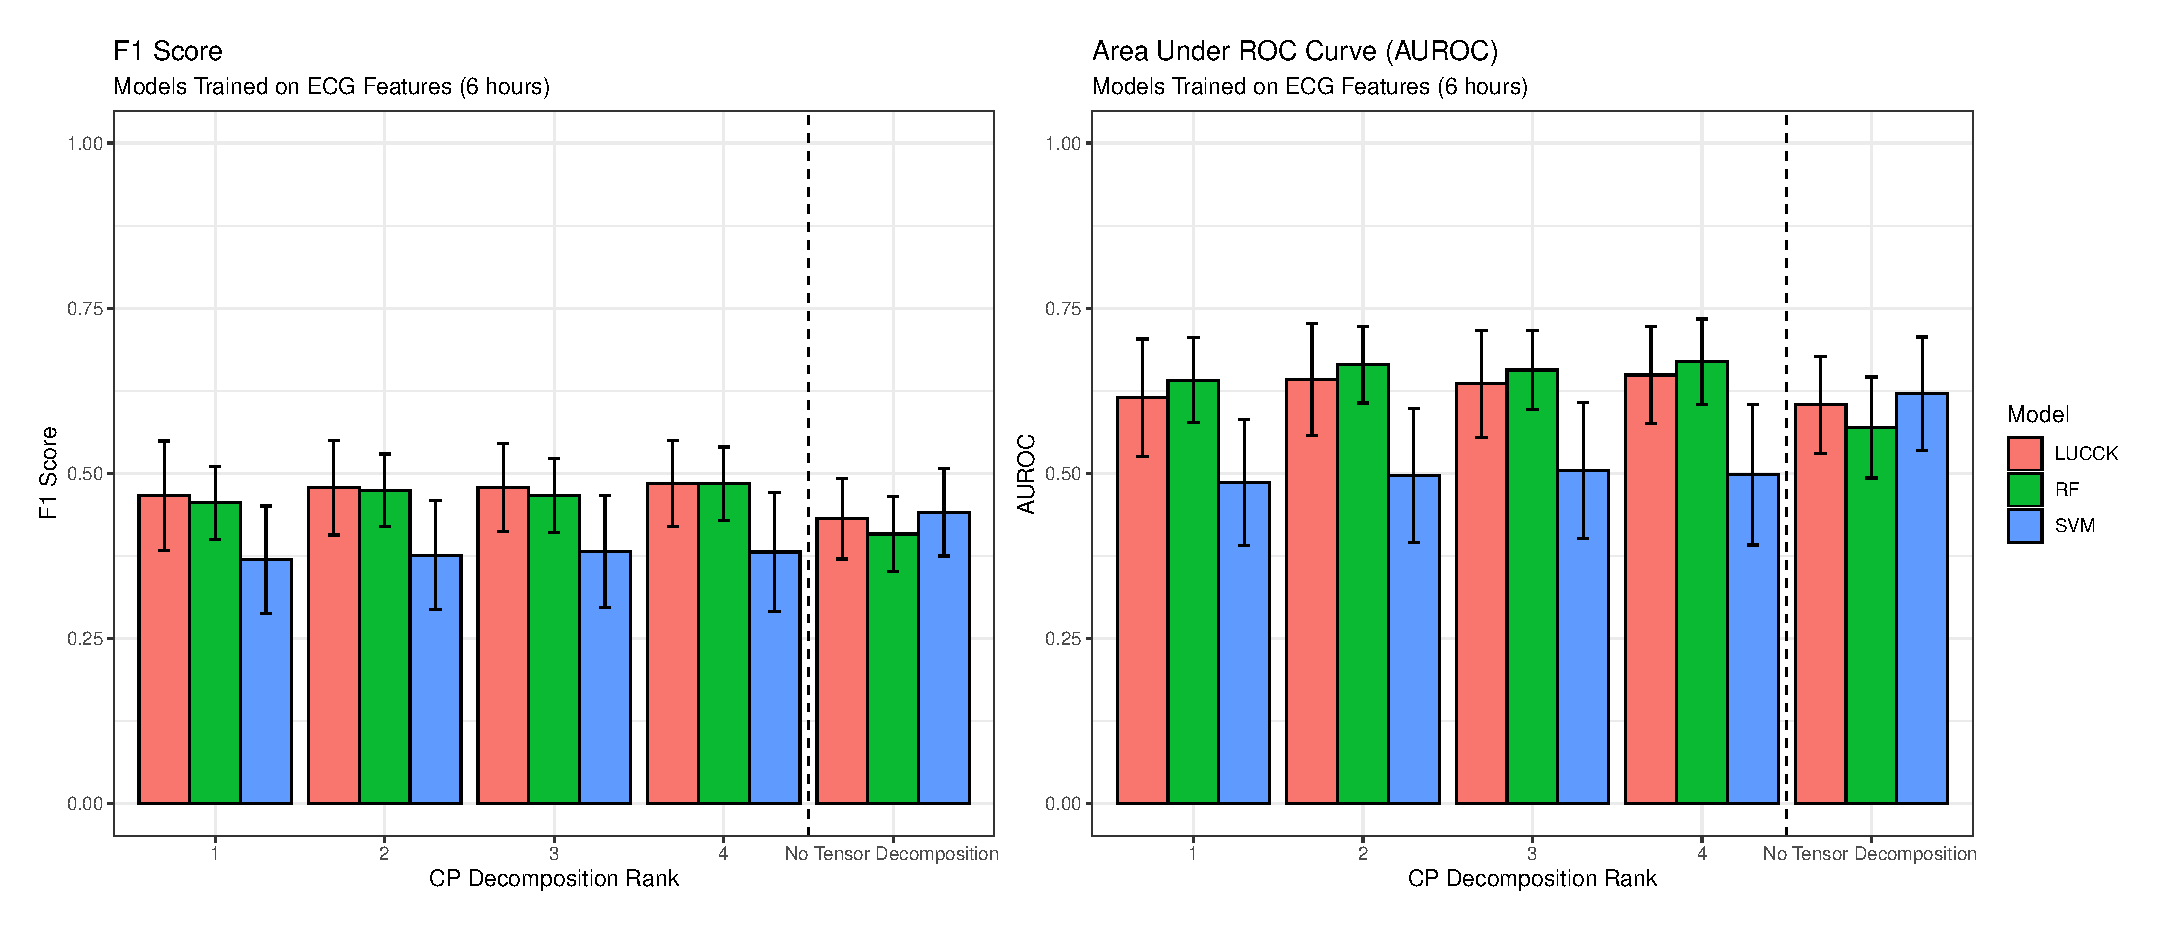
\includegraphics[width=\textwidth]{body/figures/ecg_6.eps}
        \caption{6-hour data}
    \end{subfigure}
    \hfill
    \begin{subfigure}[htb]{\textwidth}
        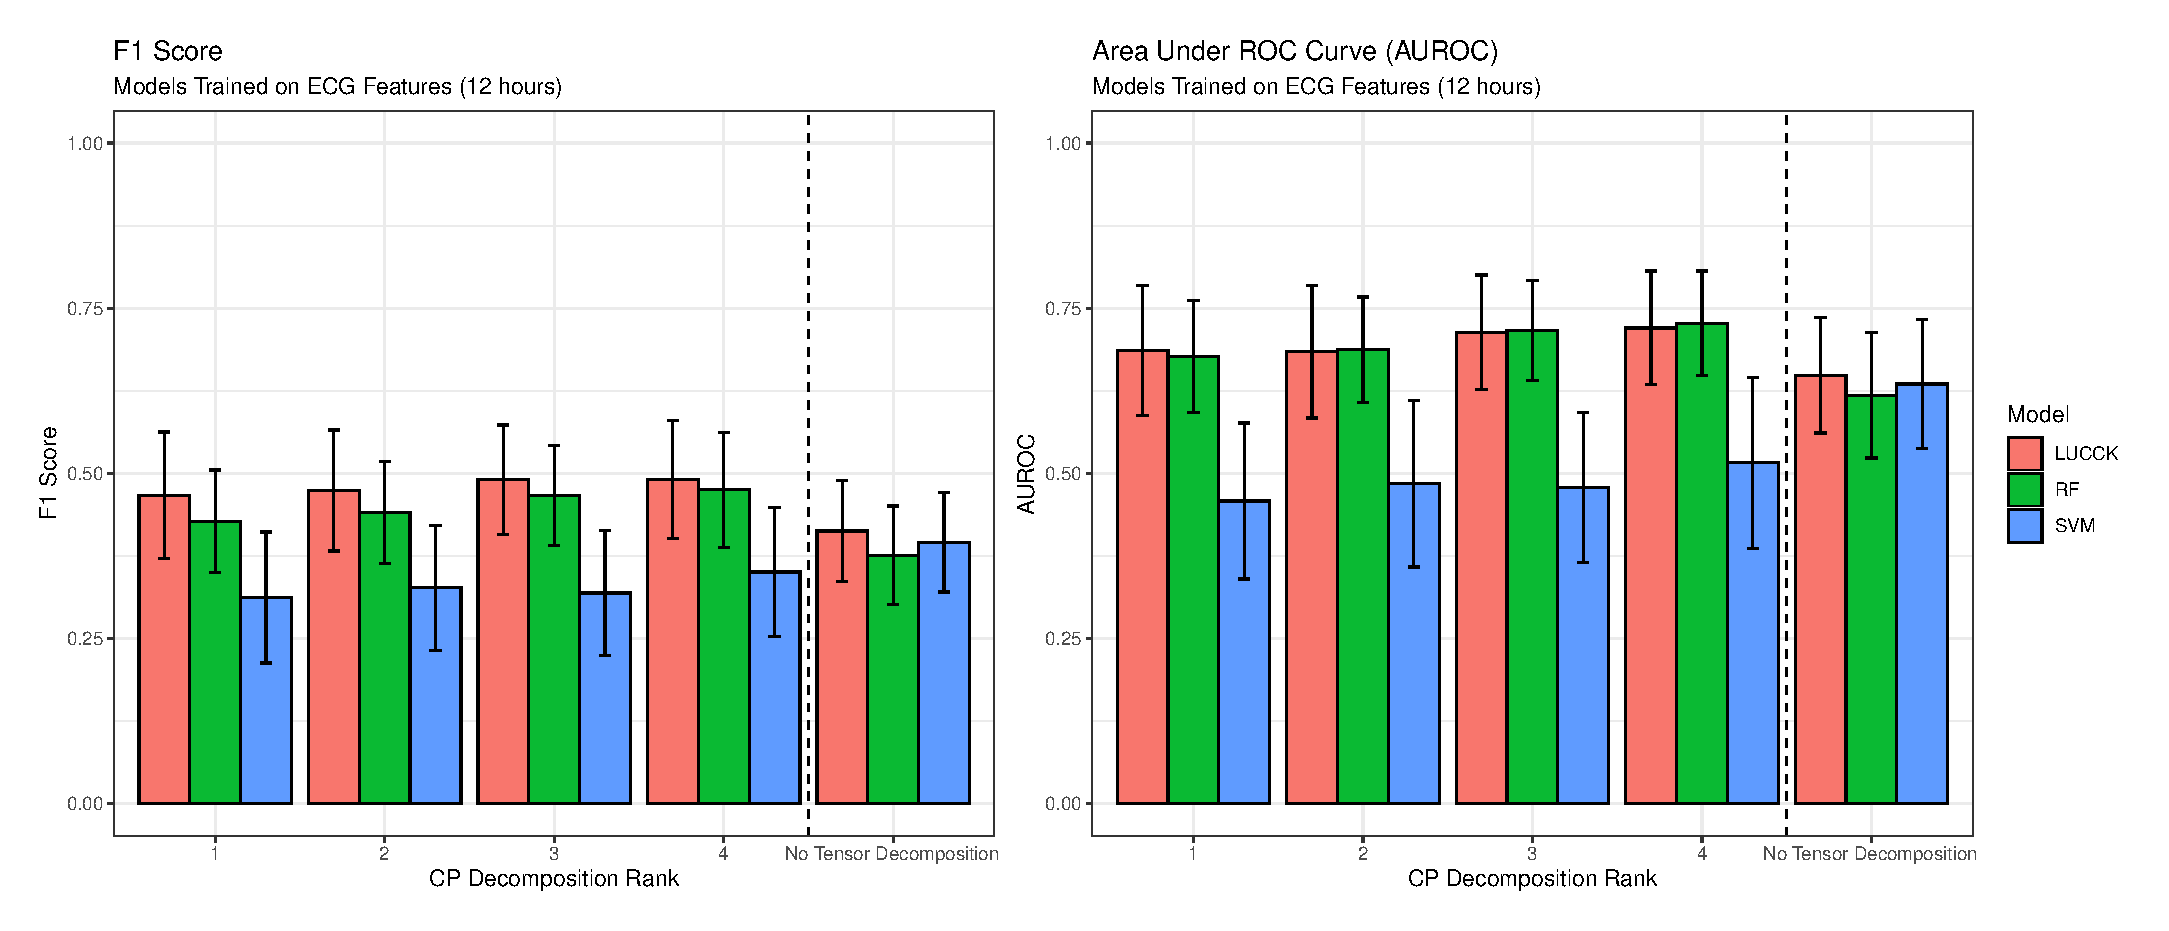
\includegraphics[width=\textwidth]{body/figures/ecg_12.eps}
        \caption{12-hour data}
    \end{subfigure}
    \caption{Models Trained with ECG}
    \label{fig:ecgonly}
\end{figure}  % ECG 

\begin{figure}[htb]
    \centering
    \begin{subfigure}[htb]{\textwidth}
        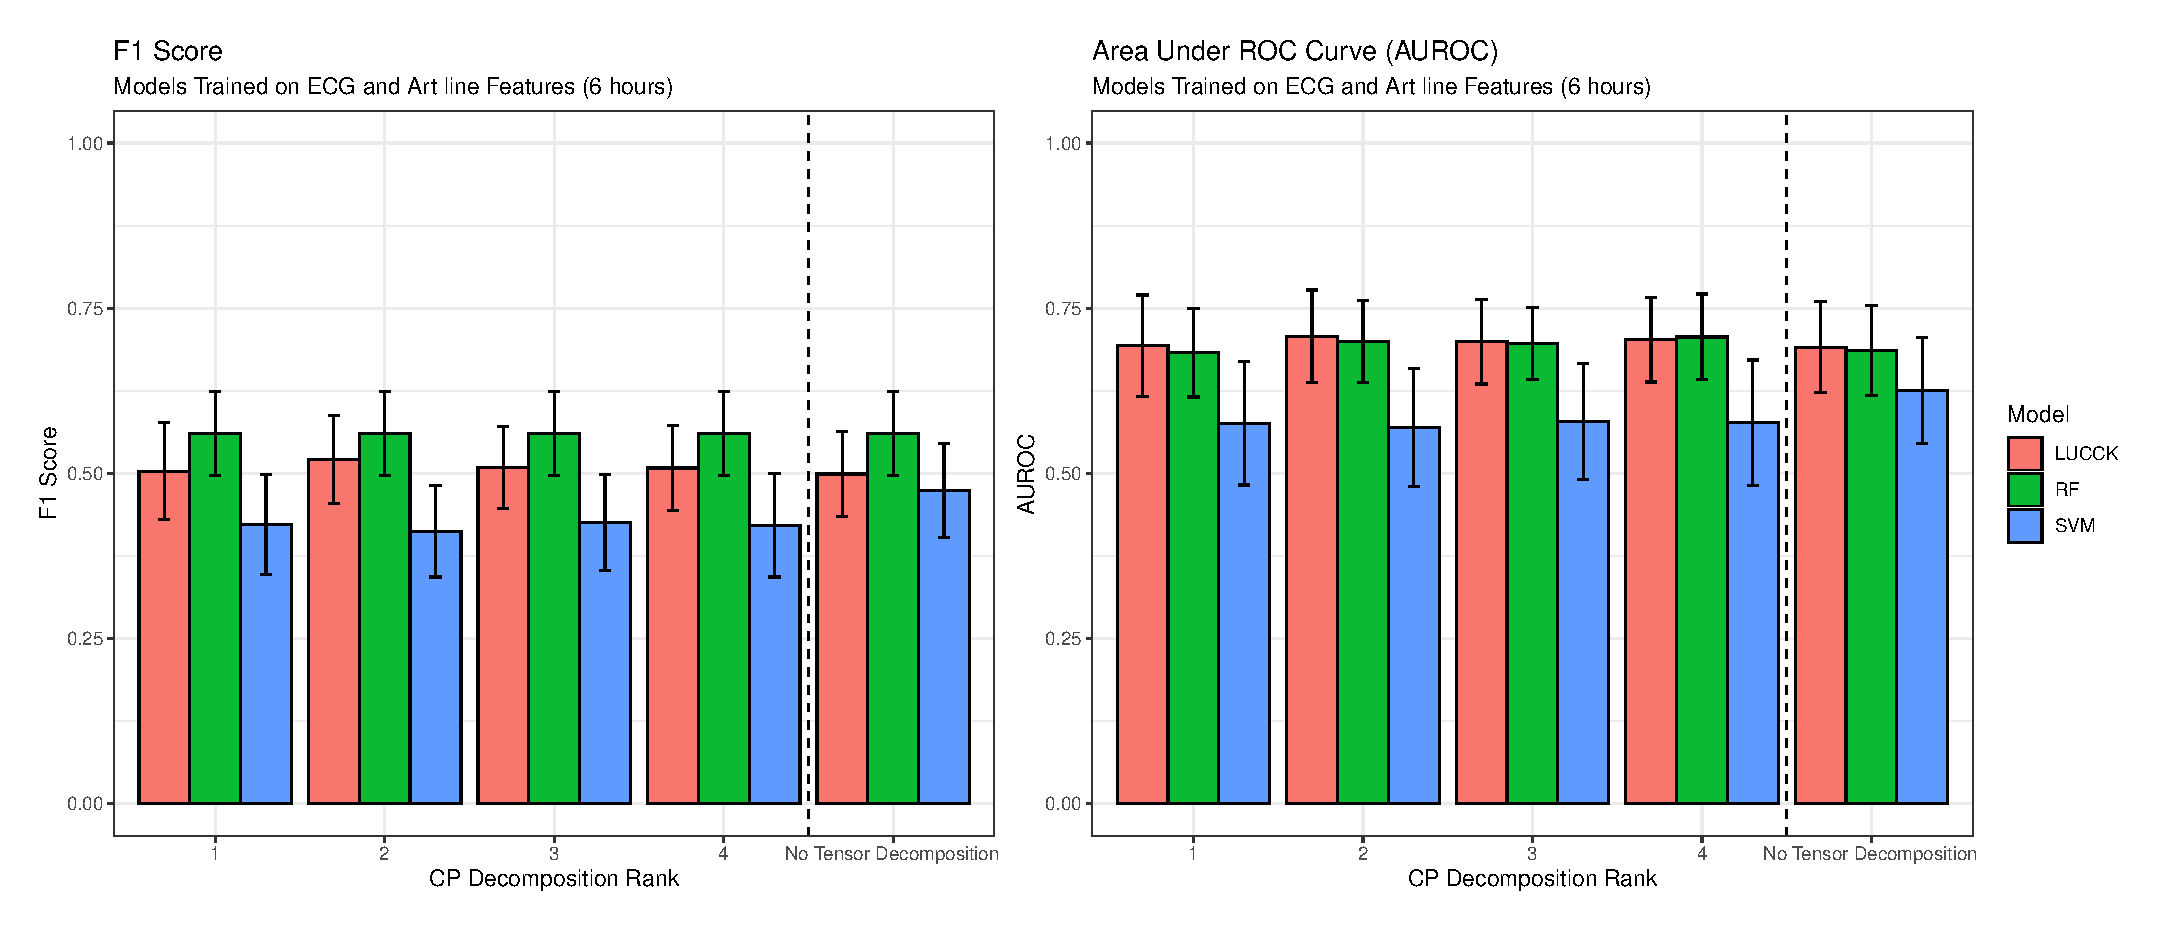
\includegraphics[width=\textwidth]{body/figures/both_6.eps}
        \caption{6-hour data}
    \end{subfigure}
    \hfill
    \begin{subfigure}[htb]{\textwidth}
        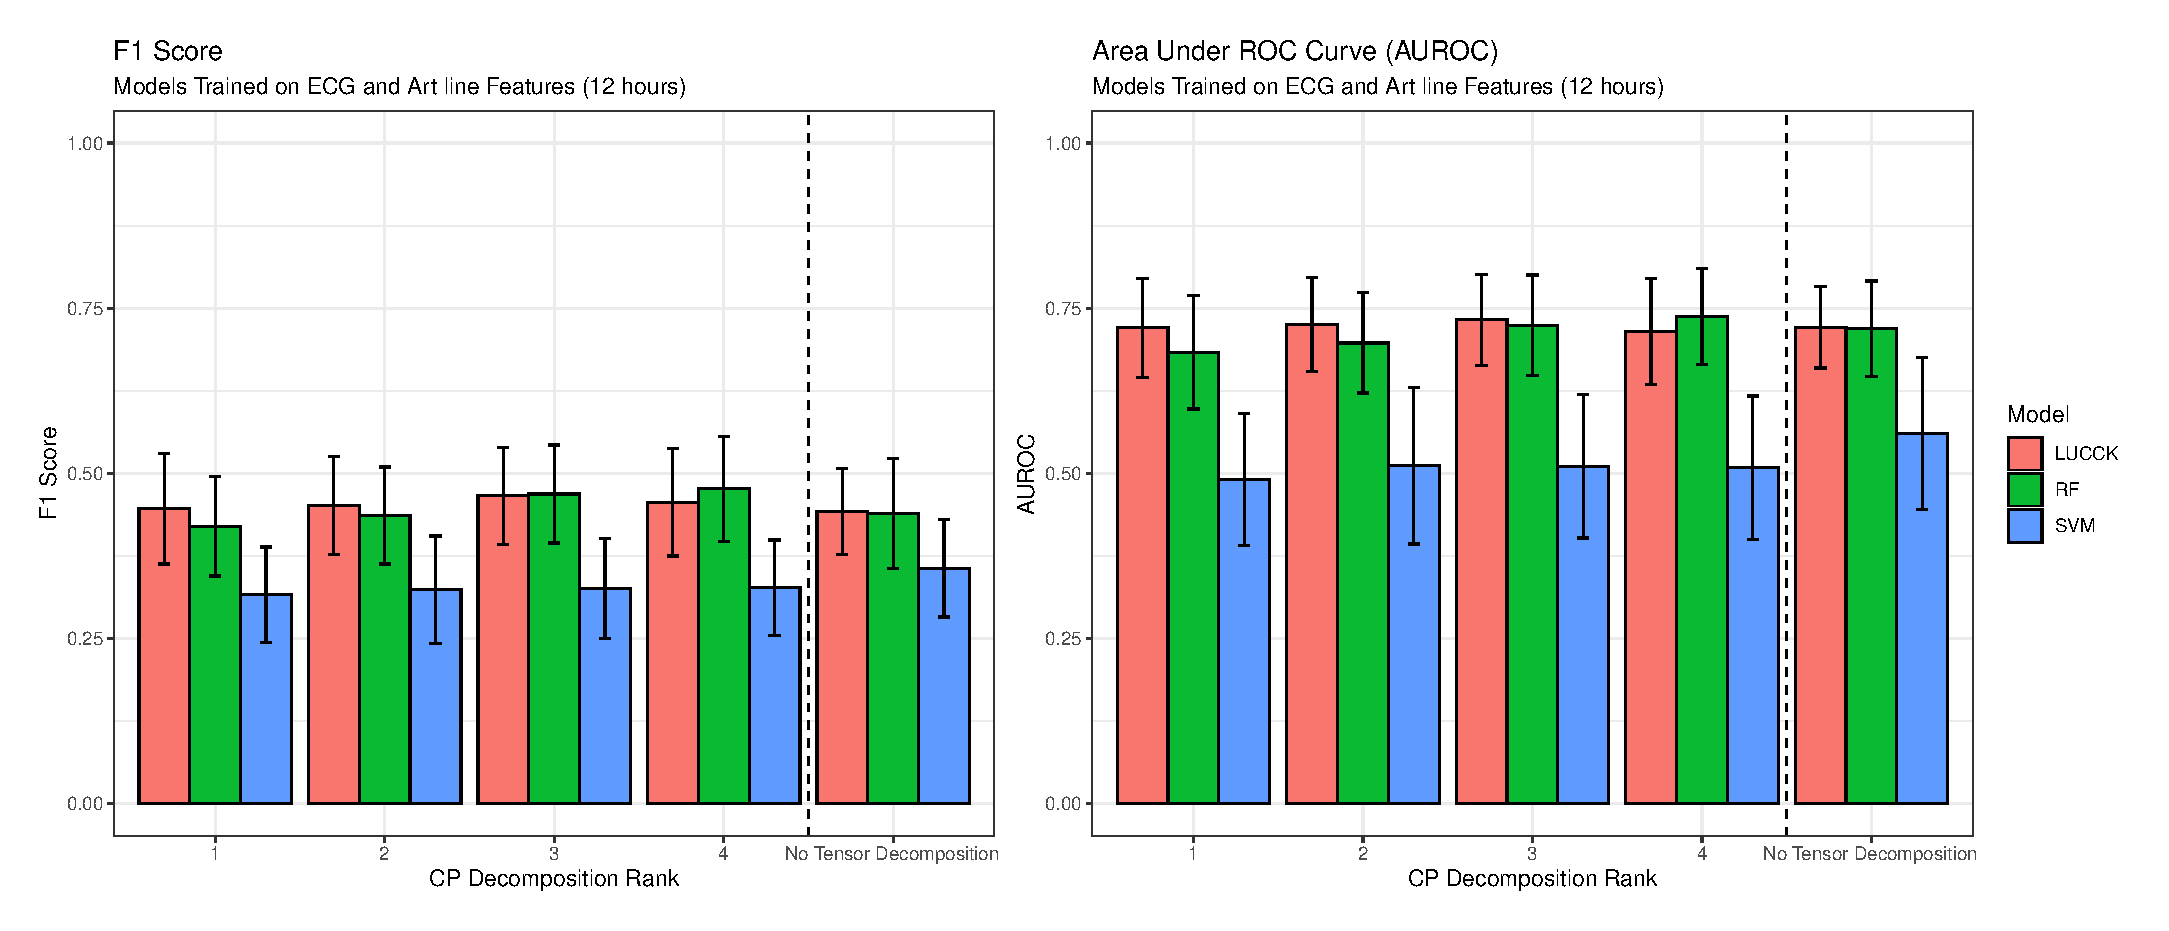
\includegraphics[width=\textwidth]{body/figures/both_12.eps}
        \caption{12-hour data}
    \end{subfigure}
    \caption{Models Trained with Arterial Line and ECG}
    \label{fig:sigonly}
\end{figure}  % ART + ECG 

\begin{figure}[htb]
    \centering
    \begin{subfigure}[htb]{\textwidth}
        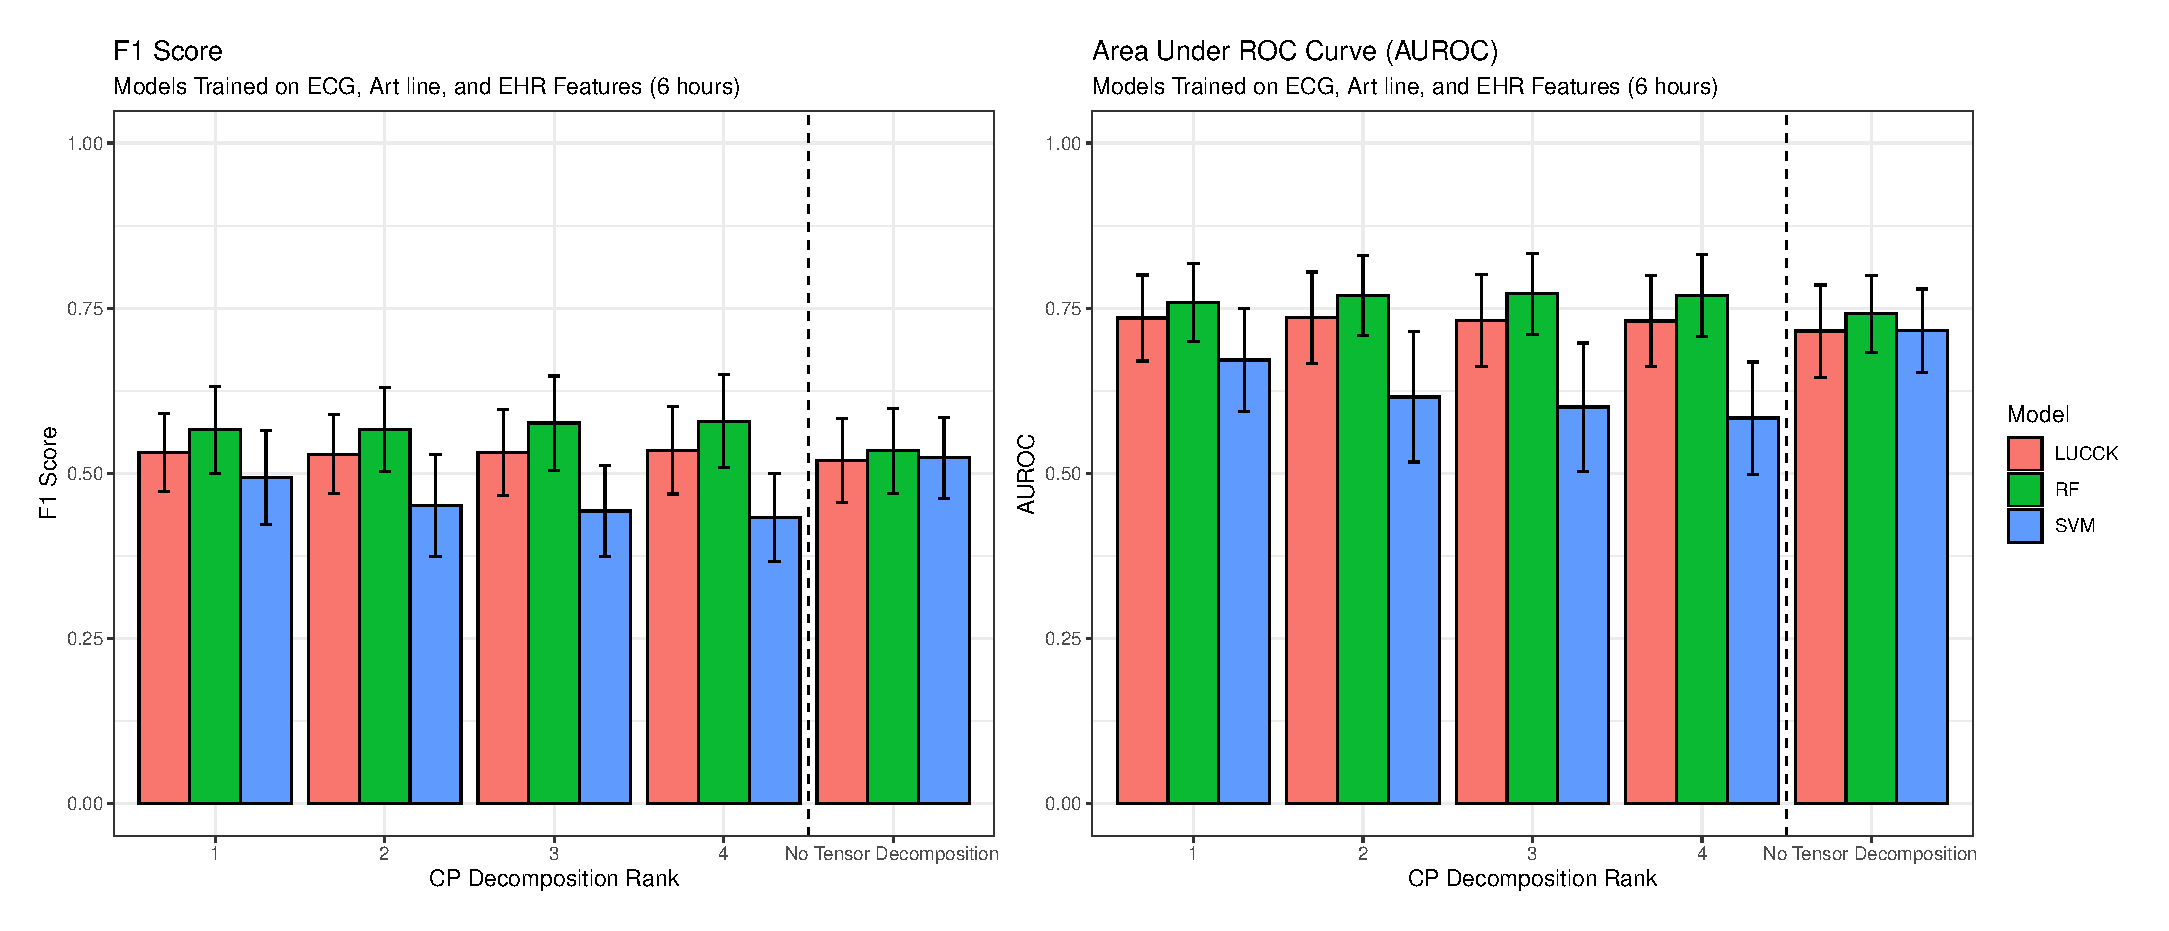
\includegraphics[width=\textwidth]{body/figures/all_6.eps}
        \caption{6-hour data}
    \end{subfigure}
    \hfill
    \begin{subfigure}[htb]{\textwidth}
        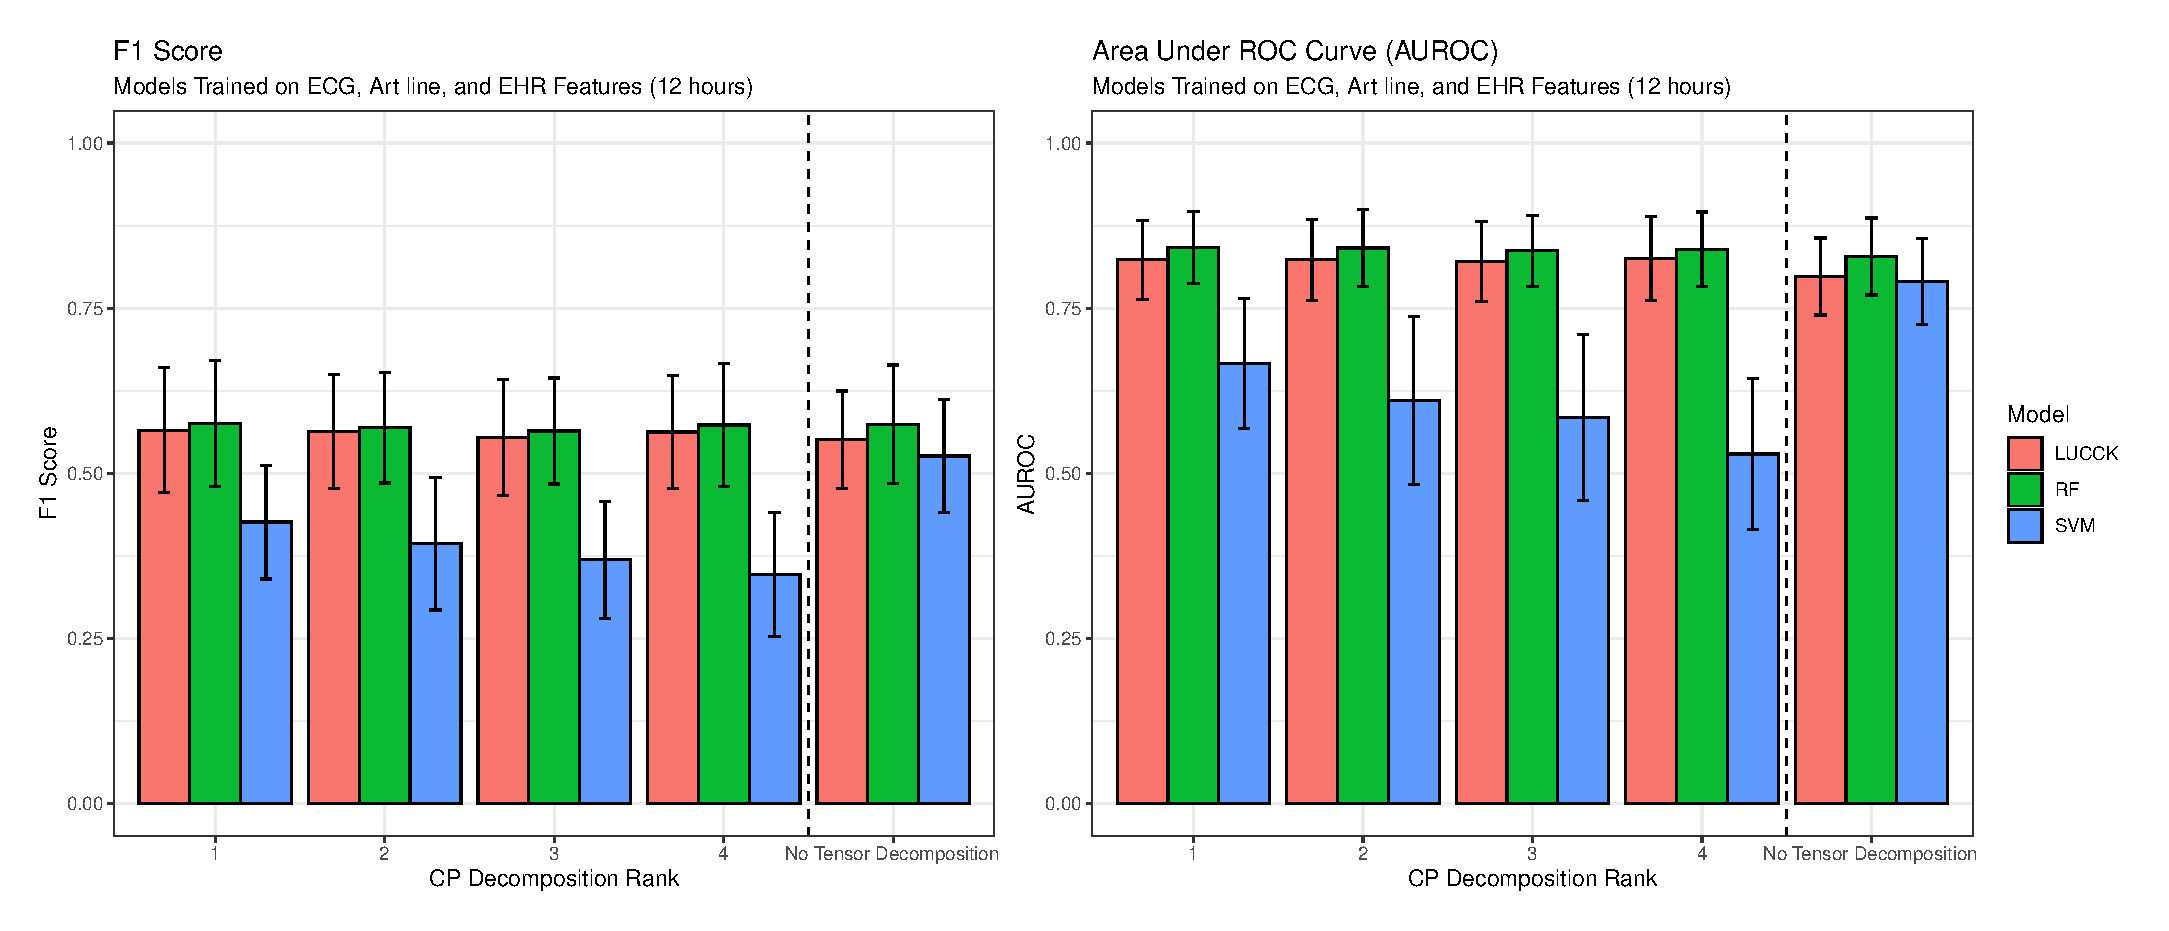
\includegraphics[width=\textwidth]{body/figures/all_12.eps}
        \caption{12-hour data}
    \end{subfigure}
    \caption{Models Trained with Arterial Line, ECG, and EHR Data}
    \label{fig:sigEHR}
\end{figure}  % ART + ECG + EHR 

\clearpage
    
    \section*{Discussion} \label{sec:discussion}
    % This should explore the significance of the results of the work, not repeat them. A combined Results and Discussion section is often appropriate. Avoid extensive citations and discussion of published literature.

RF and LUCCK models performed similarly across different experiments, both performing better than SVM when tensor reduction was applied to the dataset. RF's improvement in performance could be due to its inherent ability to select subsets of features and determine feature importance. In turn, if the data are not easily linearly separable, linear SVM may struggle.
% TODO: from Gil "what do you mean by inherent ability? Relate this to 'only pertinent information and noise removal' in conclusion"

For RF and LUCCK, both F1 Score and AUROC tended to increase when moving from no tensor reduction to tensor reduction. For example, for LUCCK in the 6-hour dataset, mean F1 score increased from 0.4313 to 0.4844 with SD remaining similar (0.0612 to 0.0650), while RF's F1 score increased from 0.4080 to 0.4839 with SD decreasing from 0.0570 to 0.0558. We observed a similar increase in mean AUROC for LUCCK (0.6038 $\pm$ 0.0735 to 0.6489 $\pm$ 0.0732) and RF (0.5693 $\pm$ 0.0764 to 0.6690 $\pm$ 0.0644) going from using no tensor reduction to using CP-ALS with rank 4. SVM does not follow this trend, however, and tends to increase in performance as more information is added to the model, with no tensor reduction performing the best.

For 6-hour data, including the arterial line features improved both mean F1 Score and mean AUROC across different CP-ALS ranks, as can be seen comparing Figures \ref{fig:ecgonly} and \ref{fig:sigonly}. For 12-hour data, RF and LUCCK see some increase in performance across the different ranks, but including both Arterial Line and ECG data decreased SVM's performance when no tensor reduction took place. When CP-ALS was used with ranks 1-3 to reduce the feature space for SVM, there is an increase in performance in the ECG + Arterial Line scenario; this suggests that SVM may not be a reliable model for these scenarios.

Adding EHR data to the signal features, presented in Figure \ref{fig:sigEHR}, further improves performance for both the 6- and 12-hour datasets, across all three model types.

While the results of models trained on tensor-reduced signal features show consistent mean AUROC $\geq$ 0.6500 for both LUCCK and RF, it is noted that these experiments were trained on data from only one hospital, the availability of signals led to a small sample pool, and the datasets used do not feature strong racial and ethnic diversity. To ensure the reproducibility and generalizability of these results, it will be necessary to perform similar experiments on a larger and more diverse dataset in future iterations.


    
    \section*{Conclusion} \label{sec:conclusion}
    % The main conclusions of the study may be presented in a short Conclusions section, which may stand alone or form a subsection of a Discussion or Results and Discussion section.

% jonathan: rewrite to match changes to abstract
In this study, predictions of increase in qSOFA score were created using tensor-reduced signal features and EHR data. It is possible to make a prediction of increase in qSOFA score using ECG data alone (for RF, AUROC 0.6690 $\pm$ 0.0644; for LUCCK, 0.6489 $\pm$ 0.0732), and results can be improved if tensor-reduced arterial line features are added, (for RF, AUROC 0.7064 $\pm$ 0.0650; for LUCCK, 0.7073 $\pm$ 0.0700), but results are mixed when signal features are directly added without tensor reduction (for RF, AUROC 0.6855 $\pm$ 0.0650; for LUCCK, 0.6906 $\pm$ 0.0689). This may be because the models are overwhelmed with information, whereas tensor reduction improves performance because only pertinent information is given and noise is removed. 

The previous experiments simulate the scenario when no EHR data is available. When EHR data is available and CP-ALS is used to reduce the feature space of the signal data, results can be further improved (for RF, AUROC 0.7691 $\pm$ 0.0617; for LUCCK, 0.7305 $\pm$ 0.0689). This indicates that ECG signal features, Arterial Line signal features, and EHR data features can all contribute to sepsis prognosis. 

That said, we wish to draw attention to the first scenario, with signals information alone used for model training. The advantage of a signal features-based model is that predictions can be made in the ICU on a continuous basis in real-time; this model would not be limited by the wait times or availability of EHR data variables. From a clinical standpoint, further developing an ECG-only model would be advantageous as, one, it is minimally invasive compared to an arterial line, and two, it is possible to monitor ECG remotely outside the hospital. Devices such as Holter monitors and Zio patches could be used so that a patient with initially low qSOFA could be monitored at home, with a 6-hour window to predict an increased risk for poor outcomes. Six hours would be adequate time for warning and arrival to the emergency department to seek appropriate treatment.

% jonathan: Think about other strengths and limitations that should be added
We stress that, while it may not achieve F1 or AUROC scores as high as the model including EHR data, our signal features-only model offers an advantage in that it is not prone to issues such as availability or inaccuracies of EHR data. Furthermore, it is continuously collected allowing for real-time evaluation and assessment. For future work, we recommend (1) the combination of EHR, tensor-reduced ECG, and tensor-reduced arterial line for use in the hospital or ICU and (2) tensor-reduced ECG only for use in home monitoring.
    
    \section*{Contributors}
    JG, JSV, KN, and OPA conceptualised and designed the study. HD developed the code and algorithms for performing peak detection. HD, SC, and JP developed the method and code for tensor methods and dimensionality reduction. JG confirmed access to and verified the dataset used in this study. JSV and GO provided clinical knowledge. OPA performed feature extraction and developed the models. WZ developed the algorithm and code to perform the quality check of electrocardiogram data. All authors have discussed the results and contributed to the final manuscript.
    
    \section*{Conflict of Interest Statement}
    KN, JG, and HD have intellectual property with University of Michigan's Office of Technology Transfer related to the content of this paper.
    
    \section*{Role of the Funding Source}
    All aspects of this research were supported by the NSF grant no. 1837985. The NIH training grant no. T32GM070449 supported OPA and WZ. We also acknowledge NIH grants 3-P30-ES-017885-11-S1 and 3-U24-CA-271037-02-S1. 
The content is solely the responsibility of the authors and does not necessarily represent the official views of the National Institutes of Health.

    \section*{Data Availability}
    The data that support the findings of this study belong to the University of Michigan, and cannot be publicly distributed due to reasons of patient privacy. Data are located in controlled access data storage at the University of Michigan. De-identified data supporting this study may be shared based on reasonable written request, which will be considered by the University of Michigan.

    
    \printbibliography 

\end{document}
